\begin{frame}
    \frametitle{Enriched uranium masses}
    \begin{table}
        \centering 
        \caption{Metrics for enriched uranium sent to advanced 
        reactors between 2025-2090 in Scenarios 2-7.}
        \label{tab:nogrowth_uranium}
        \begin{tabular}{l p{2cm} p{2cm} p{2cm} p{2cm}}
            \hline
            Scenario & Average (MT/month) & \gls{HALEU} Average 
            (MT/month) & Maximum (MT)& Cumulative (MT)\\\hline
            2 & 88.90 & 88.90 & 1,007 & 69,251\\
            3 & 31.64 & 31.64 & 86.79 & 24,646\\
            4 & 33.62 & 33.62 & 101.5 & 26,193\\
            5 & 152.3 & 3.070 & 581.1 & 118,608\\
            6 & 39.92 & 29.51 & 103.3 & 31,095\\
            7 & 33.85 & 32.97 & 103.0 & 26,370\\
            \hline
        \end{tabular}
    \end{table}
\end{frame}

\begin{frame}
    \frametitle{SWU capacity}
    \begin{table}
        \centering 
        \caption{Metrics for \gls{SWU} capacity to enrich uranium for 
        advanced reactors between 2025-2090 in Scenarios 2-7.}
        \label{tab:nogrowth_swu}
        \begin{tabular}{l p{2cm} p{2cm} p{2cm}}
            \hline
            Scenario & Average  (MT-SWU/month) & Average
            for \gls{HALEU} (MT-SWU/month) & Maximum (MT-SWU)\\\hline
            2 & 4,010 & 4,010 & 45,424 \\
            3 & 1,090 & 1,090 & 2,991\\
            4 & 1,192 & 1,192 & 3,668\\
            5 & 1,145 & 138.5 & 4,228 \\
            6 & 1,087 & 1,017 & 3,050\\
            7 & 1,167 & 1,161 & 3,735\\
            \hline
        \end{tabular}
    \end{table}
\end{frame}

\begin{frame}
    \frametitle{SNF discharged}
    \begin{table}
        \centering 
        \caption{Metrics for waste discharged from advanced reactors 
        between 2025-2090 in Scenarios 2-7.}
        \label{tab:nogrowth_waste}
        \begin{tabular}{l p{2cm} p{2cm} p{2cm} p{2cm}}
            \hline
            Scenario & Average (MT/month) & Average of \gls{HALEU} 
            (MT/month) & Maximum (MT) & Cumulative (MT)\\\hline
            2 & 66.15 & 66.15 & 1,142 & 51,531\\
            3 & 32.93 & 32.93 & 55.29 & 25,654\\
            4 & 34.07 & 34.07 & 77.55 & 26,543\\
            5 & 144.9 & 2.294 & 377.0 & 112,913\\
            6 & 40.68 & 30.72 & 75.12 & 31,691\\
            7 & 34.46 & 33.62 & 83.14 & 26,848\\
            \hline
        \end{tabular}
    \end{table}

\end{frame}

\begin{frame}
    \frametitle{Transition Start Time}
    \begin{figure}
        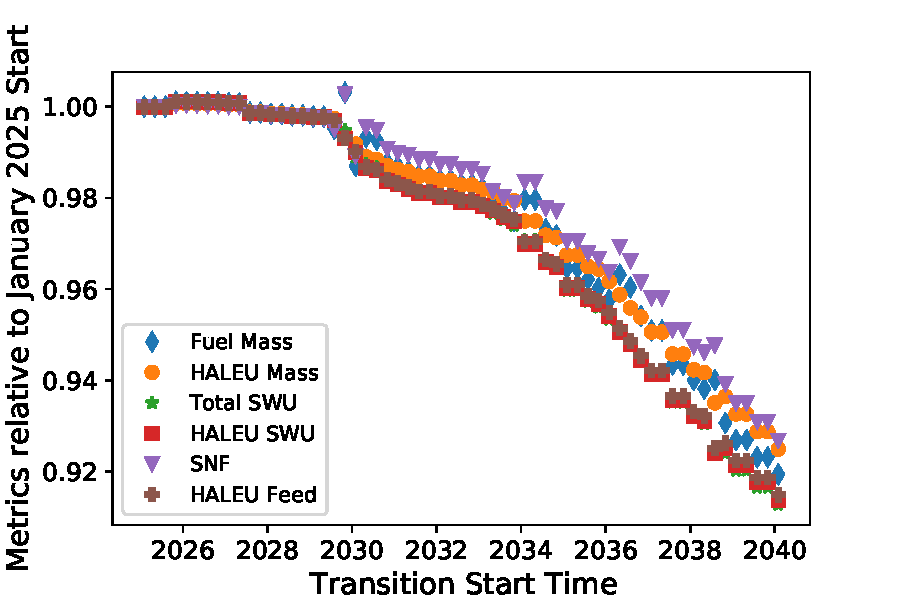
\includegraphics[scale=0.5]{ts.pdf}
        \caption{Change in metrics from varying the transition start time.}
        \label{fig:ts}
    \end{figure}
\end{frame}

\begin{frame}
    \frametitle{LWR Lifetime}
    \begin{figure}
        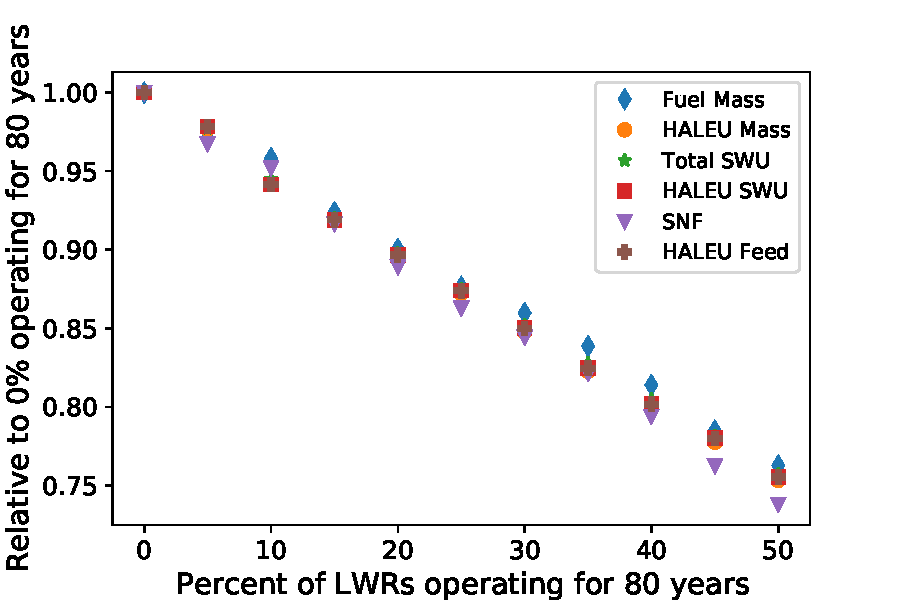
\includegraphics[scale=0.5]{lwr.pdf}
        \caption{Change in metrics from varying the percent of 
        the LWR fleet operating for 80 years.}
        \label{fig:lwr}
    \end{figure}
\end{frame}

\begin{frame}
    \frametitle{MMR Burnup}
    \begin{figure}
        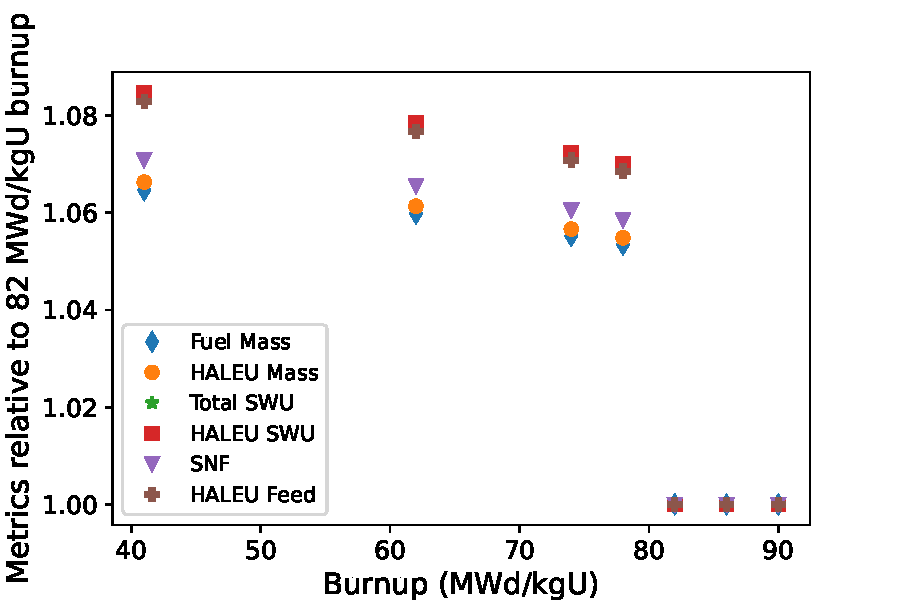
\includegraphics[scale=0.5]{mmr_bu.pdf}
        \caption{Change in metrics from varying the MMR burnup.}
        \label{fig:mmr_bu}
    \end{figure}
\end{frame}


\begin{frame}
    \frametitle{Xe-100 burnup}
    \begin{figure}
        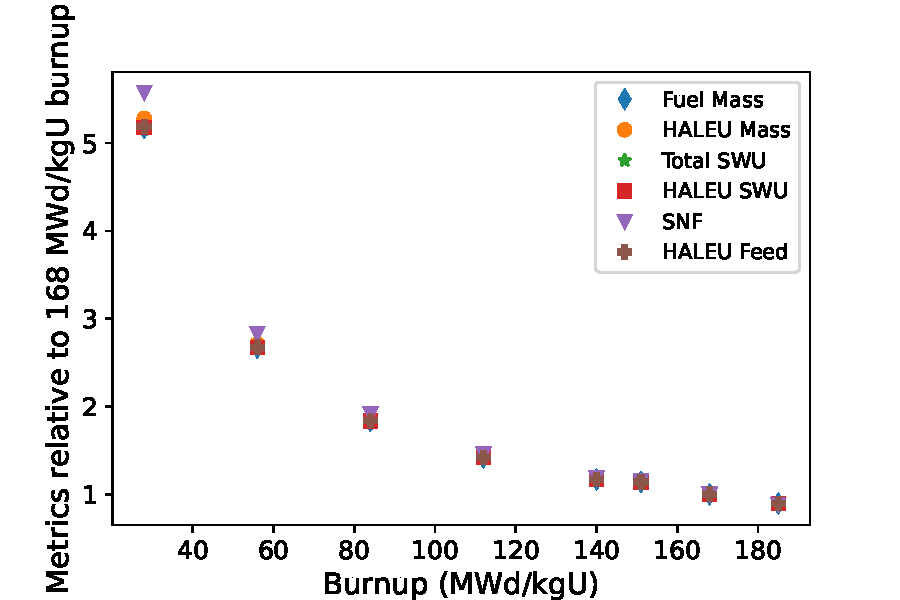
\includegraphics[scale=0.5]{xe100_bu.pdf}
        \caption{Change in metrics from varying the Xe-100 burnup.}
        \label{fig:xe100_bu}
    \end{figure}
\end{frame}

